\documentclass[a4paper,11pt,twoside]{article}

%===========PACOTES
\usepackage[body={170mm,235mm}]{geometry}
%\usepackage[portuguese]{babel}
\usepackage{a1}
\usepackage[english]{babel}
\usepackage[latin1]{inputenc} %permite o uso de acentos
%\usepackage[dvips]{color}
\usepackage{amsfonts,amssymb}
%\usepackage{epsfig}
\usepackage{amsmath}
\usepackage{graphicx}	

% makeidx
\usepackage{makeidx}
% make index
\makeindex
%\usepackage[pdftex]{graphicx}


\def\mapright#1#2#3{\smash{\mathop{\hbox to
#3{\rightarrowfill}}\limits^{#1}_{#2}}}

\def\mapleft#1#2#3{\smash{\mathop{\hbox to
#3{\leftarrowfill}}\limits^{#1}_{#2}}}

\def\mapright#1#2{\smash{\mathop{\hbox to 0.90cm{\rightarrowfill}}\limits^{#1}_{#2}}}
\def\mapleft#1#2{\smash{\mathop{\hbox to 0.90cm{\leftarrowfill}}\limits^{#1}_{#2}}}

\def\mapleftright#1#2{\smash{\mathop{\hbox to 0.80cm{\leftarrowfill \rightarrowfill}}\limits^{#1}_{#2}}}
\def\ext{\times \! \vrule depth0pt height5pt width0.35pt}

\def\H{\mathcal H}
\def\D{\mathcal D}
\def\B{\mathcal B}
\def\C{\mathbb C}
\def\R{\mathbb R}
\def\S{\mathbb S}
\def\U{\mathcal U}
\def\Z{\mathbb Z}

\title{All the shapes of spaces: a census of small 3-manifolds
\footnote{2010 Mathematics Subject Classification: 
57M25 and 57Q15 (primary), 57M27 and 57M15 (secondary)}} 
\author{S�stenes L. Lins and Lauro D. Lins}

\date{\today}


\begin{document}


\maketitle
\begin{abstract}


In this work we present a complete (no misses, no duplicates) catalogue for closed, 
connected, orientable and
prime 3-manifolds induced by plane graphs with a 
bipartition of its edge set (blinks) up to 9 edges. Blinks form a universal encoding for such manifolds. 
We hope that this census becomes as useful for the study of concrete examples of 3-manifolds
as the tables of knots are in the study of knots and links. 

% Along the years we have made an issue
% in our computational work that it must be reproducible and independently checked by other researchers. 
% Our software {\sf BLINK} is available,
% but currently it lacks yet a good documentation and help is welcome to change this. 
% An Wiki open source project is starting.


\end{abstract}


\section{Introduction} 



After presenting some instances of closed 3-manifolds,
P. Alexandroff says in the English translation (1961) of 
his joint work with D. Hilbert \cite{alexandrov1961elementary}, first
published (1932) in German, \cite{alexandroff1932einfachste}:
{\em ``These few examples will suffice. Let it be remarked here that, at present,
in contrast with the two-dimensional case, the problem of enumerating the 
topological types of manifolds of three and more dimensions is in an apparently 
hopeless state. We are not only far removed from the solution, but even from the first step
toward a solution, a plausible conjecture''.}


John Hempel in his book (1976) {\em 3-Manifolds} \cite{hempel1976} writes 
at the opening of Section 15, entitled {Open Problems:}
{\em ``The ultimate goal of the theory would be in providing solutions to:
 {\em The homeomorphism problem}: provide an {\em effective} procedure
 for determining whether two {\em given} 3-manifolds are homeomorphic, together with
 {\em The classification problem}: {\em effectively} generate a list containing
 exactly one 3-manifold from each homeomorphism class.''}

 
 It is amazing how much the picture has changed in the 80 years since Alexandroff's-Hilbert book.
 The progress was due to the deep advances in the 1950's and 1960's, starting with
 the proof that 3-manifolds are triangulable by Moise (1952), \cite{moise1952affine}. Next 
 the presentation
 of them by framed links by Lickorish (1962) \cite{lickorish1962representation}.
 Following that Kirby presented its calculus for framed links (1978)\cite{kirby1978calculus}. 
 starting in the early 1980's W. Thurston's breakthroughs, developing his conceptual theory 
 on hyperbolic manifolds and of the geometrization conjecture. 
 In the final 1980's early 1990's Witten \cite{witten1989quantum} broke the psicological 
 barrier that there were no good invariants for 3-manifolds. Following that a number of 
 eastern European mathematicians like N. Reshetikhen, V. Turaev and O. Viro, 
 \cite{turaev1992state,reshetikhin1991invariants}
 using quantum groups were able to put in mathematical solid ground Witten's findings.
 One of us, S. Lins, was a witness of the excitement these developments caused. L. H. Kauffman
 and W. B. R. Lickorish discovered the relationship of the Temperley-Lieb algebra with the new invariants,
 \cite{lickorish1991three}. Starting with a sabatical leave in to Chicago in 1990, S. Lins produced
 the joint monography with Kauffman \cite{kauffman1994tlr}, where blinks are first defined 
 and extensive WRT-invariant computations were obtained from the theory developed from scratch,
 independently and simpler than that of quantum groups.  In the early 
 2000's, G. Perelman revolutionized the field proving Poincar�'s Conjecture and
 Thurston's Geometrization Conjecture. More recently in the 2010's, I. Agol is leading the field
 in this era post-Perelman. Of course, this is only a diagonal list of researchers. Many more have contributed and
 some are  extremely active in this era pos-Perelman, \cite{friedl3}. 
 Currently there is a great amount of important reserch issues
 going on and these are exciting times for 3-manifold theory. See the recent essay of E. Klarreich
 in the Simons Foundation, \cite{Klarreich1012}.
  
 We present here our modest contribution to the topic.
 It is placed in the confluency of two deep passions of the authors:
 the study of closed orientable 3-manifolds and the study of plane 
 graphs. In this regard, see how 3-manifolds become an equivalence class of plane graphs in
 \cite{lins2013B}. Here, we mean to provide a strategy for a 
 segmented answer of Hempel's questions. 
 The closed oriented 3-manifolds are partitioned
 by the number of edges in a minimum encoding of them by a certain class of plane graphs, 
 named blinks. A {\em blink} is a finite plane graph 
 (that is already given embedded in the plane) together with an arbitrary bipartition
 of its edges into black and gray. Any closed, oriented 3-manifold is induced by some blink.
 In fact, blinks are in 1-1 correspondence with blackboard framed 
 links \cite{kauffman1991knots}, which are integer framed links capable of induce
 any such 3-manifold.
 
 Lexicography is used to define a representative unique plane graph (a canonical form) 
 for each closed oriented 3-manifold. We explicitly solve the segmented problem 
 up to 9 edges, see Theorem \ref{theorem:census9}. This work provides 
 an efficient algorithm to make available the canonical form of any closed orientable 3-manifold
 induced by plane graphs at the current level of the catalogue (currently 9 edges) and, theoretically, this
 could be extended 10, 11,\ldots, $n$, for arbitrarily large $n$. Our theory gives a road to effectively
 name each 3-manifold classified by some set of invariants $INV$. We have a universal set of object, the blinks up
 to $n$ edges, which can be partitioned by these invariants. The $INV$-classes are then tried to be broken into
 homeomorphisms classes. New invariants are then discovered and added to $INV$ making them homeomorphisms classes 
 of $n$-small manifolds. The difficult cases are going to appear naturally and they lead to enhancement of
 the theory. It is not at all impossible that this process stops and we get $INV$ so 
 that the $INV$-classes be proved to  be homeomorphisms classes for all $n$. The point we want to make is that 
 good examples (hard to find, here exemplified by the $HG12QI$ classes 
 $9_{126}$ and $9_{199}$) are important in obtaining progress in a general theory.
 A classifying $INV$ for the 9-small 3-manifolds is
 $INV=\{{\ homology}, W\hspace{-0.5mm}RT_{12}, { \ length \ of\ smallest\  geodesic}\ \}.$

\section{A complete duplicate free census of 9-small 3-manifolds}
In references \cite{kauffman1994tlr}, \cite{lins2007blink} and \cite{lins1995gca}
we have defined and show how a {\em blink}, that is, a plane graph with
an arbitrary partition of its edges (here presented as colors black and gray) induces a well
defined closed oriented 3-manifold. Moreover each such a manifold 
is induced by a blink (in fact, by infinite blinks).
An {\em $n$-small} is a closed, orientable, and prime
3-manifold is a manifold induced by a blink with at most $n$ edges.
Relative to \cite{lins2007blink} the blinks of next theorem 
have receive two additions, the representative blinks
$U[1563]$ and $U[2165]$. Also the previous HG12QI-class $6_{5}$ became 
the homemorphism class $0_1$
corresponding to $\mathbb{S}^2 \times \mathbb{S}^1$. We have decreased by 1 the numbering of the 
$HG12QI$-classes $6_{6}, 6_{7}, \ldots, 6_{20}$ become the homeomorphisms classes  $6_{5}, 6_{7}, \ldots, 6_{19}$.
This is because the HG12QI-classes $9_{126}$ and $9_{199}$ of \cite{lins2007blink} split
into two topological classes. An objective of the present work is to prove that the splitings indeed take place.

We observe that the blinks are enlarged in the appendix, showing them together with the
corresponding blackboard framed links. The notation $n_i$ attached to each blink below,
is the name of its homeomorphism class, not merely its HG12QI-class, as in \cite{lins2007blink}. 

This paper concludes the proof of the following theorem: 
\begin{theorem}[The first 489 closed orientable 3-manifolds]
Let $\mathbb{M}^3$ be a closed, oriented and prime 3-manifold induced by a blink with at most 9 edges.
Then $\mathbb{M}^3$ is homeomorphic to exactly one of the 
3-manifolds induced by the 489  blinks below. Morever all of these are pairwise non-homeomorphic.
(However being redundant, we also present the corresponding census for the blackboard framed links. These census are
enlarged in the Appendix)\\
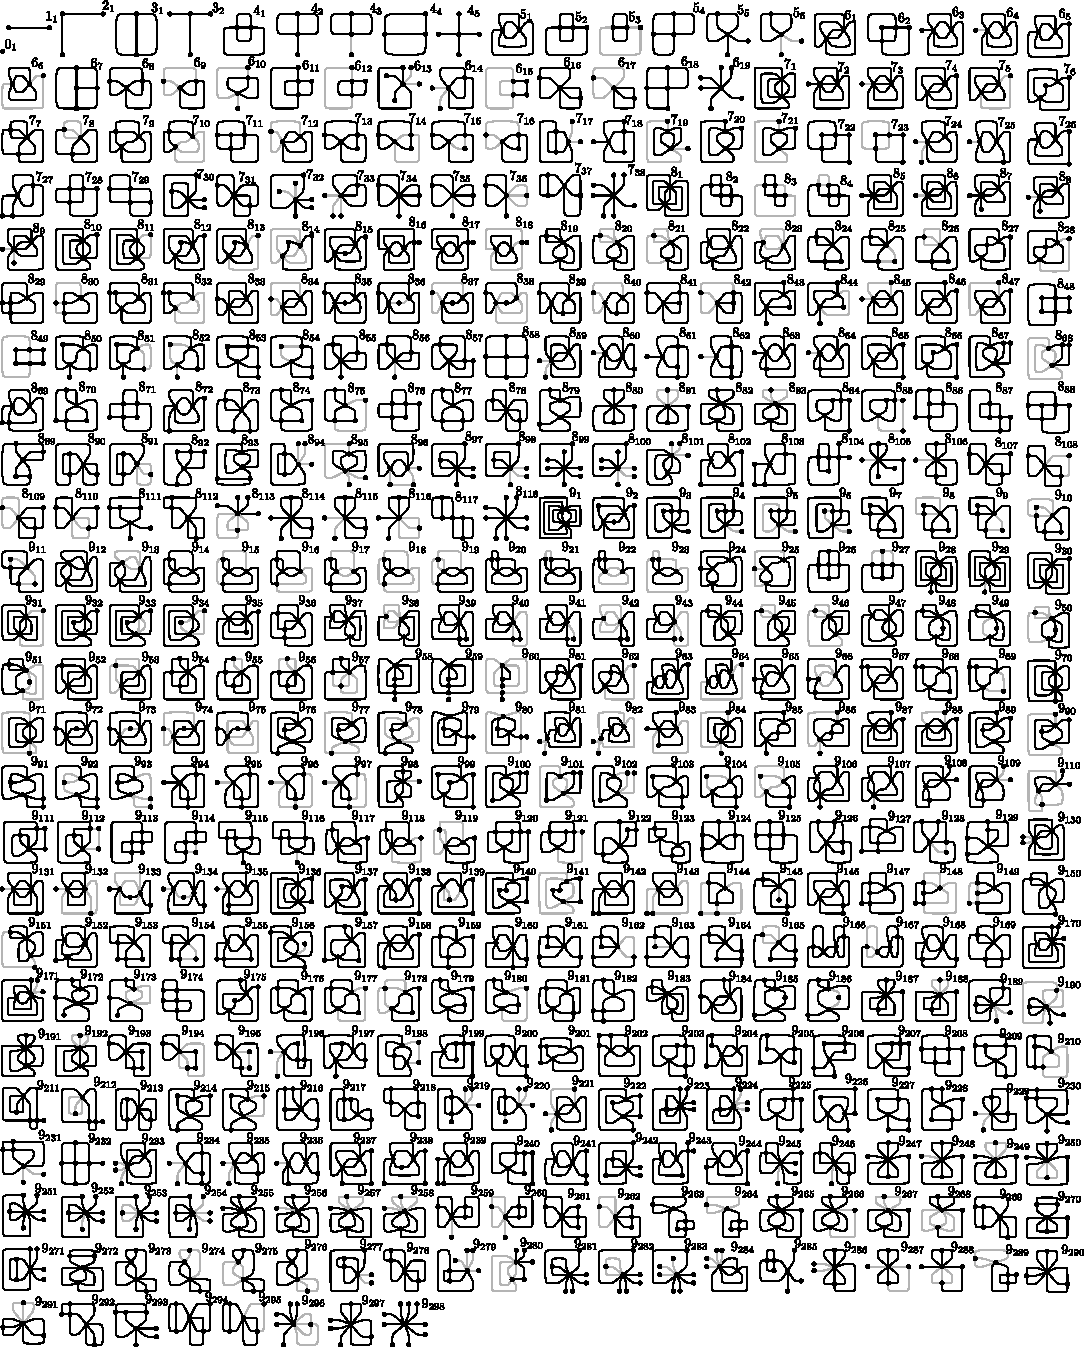
\includegraphics[width=17.5cm]{A.figs/primes489.pdf}\\
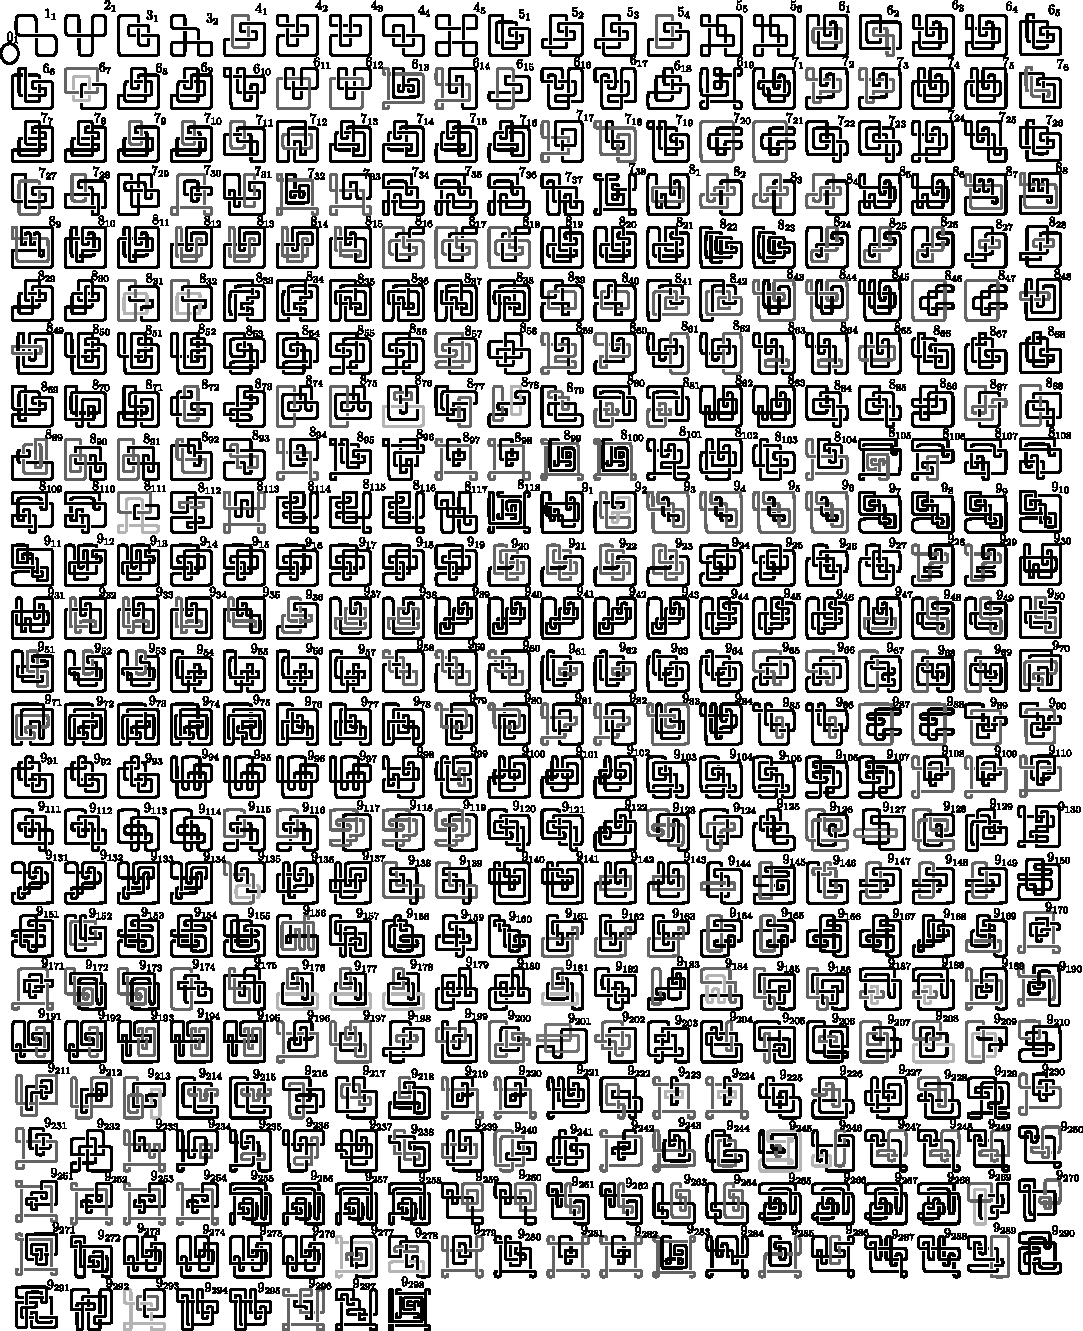
\includegraphics[width=17.5cm]{A.figs/primes489links.pdf} 
\label{theorem:census9}
\end{theorem}

\begin{proof}
 The bulk of the proof follows from L. Lins' thesis under the supervision of S. Lins, 
 \cite{lins2007blink}.
 In this work a theory of filtered blink generation is obtained 
 by pure combinatorics, lexicography and topological filtering of duplicates.
 This resulted in a set $U$ of 3437 blinks. This universal set of 9-small 3-manifold
 is partitioned by homology and WRT$_{12}$ into 487 classes, named 
 $HG12QI$-classes. 
  This is achieved by
 explicitly obtaining homeomorphisms between any two blinks in the same $HG12QI$-class.
 Here is the explanation of how each such homeomorphism can be coded into a sequence
 that is frozen in a data basis forever, and reproduced at will. 
 What remained to be done was to decide the status of the two $HG12QI$-classes
 $9_{126}$ and $9_{199}$ depicted in Fig. \ref{fig:nine126nine199}. After 7 years
 we posted these doubts as a Challenge in the arXiv, \cite{linslins2013A}. As a result,
 we got a prompty solution for the two doubts: the 3-manifolds are non-homeomorphic.
 Among other people, M. Culler, N. Dunfield and C. Hodgson sent distinct proofs of this
 fact.
 \end{proof}


\begin{figure}
\begin{center}
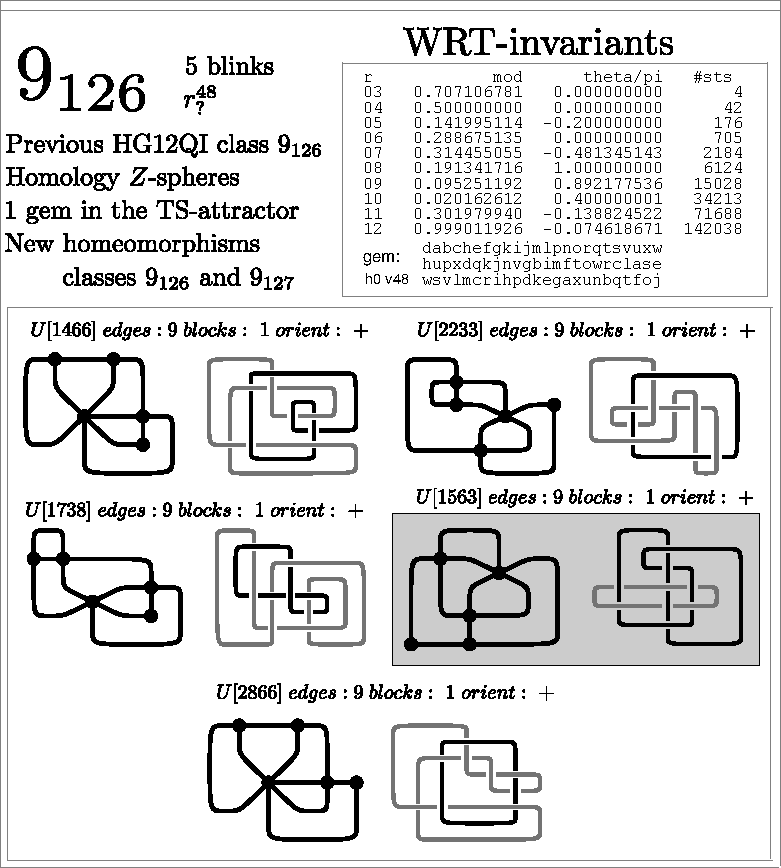
\includegraphics[width=8cm]{A.figs/nine126.pdf}
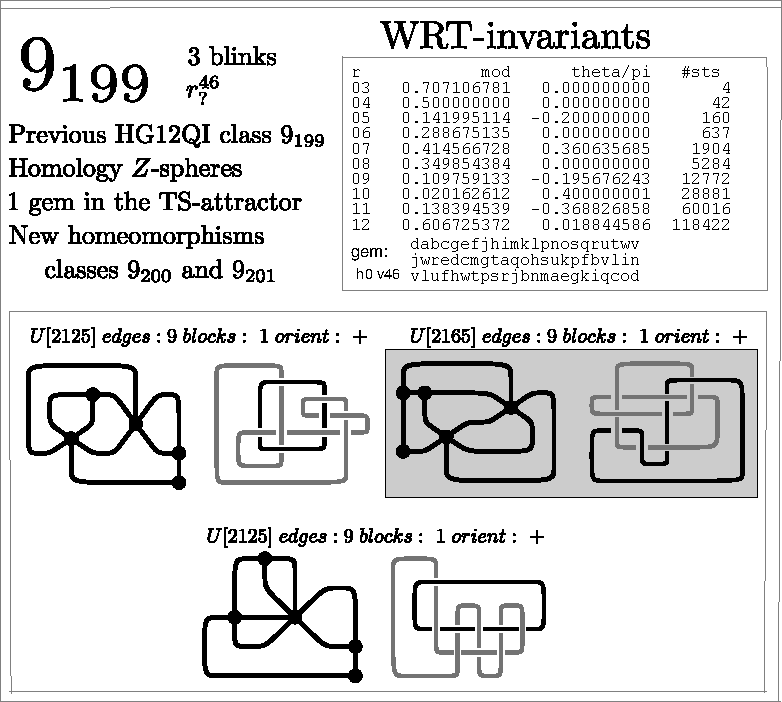
\includegraphics[width=8cm]{A.figs/nine199.pdf}
\caption{\sf The two doubts left in L. Lins's thesis are solved 
In both cases the manifolds induced
by the shaded blink-link pairs are proved very recently to be non-homeomorphic 
to the other in the same class, by geometric means. All the other pairs are proved 
to be homeomorphic by BLINK which keeps each such homeomorphism as a coded sequence which
is stored in a data basis, and, in principle reproducible at will. 
This shows that BLINK finds all available homeomorphic pairs and, in conjunction with
the length of the samllest geodesic, provides
the topological classification of the 9-small 3-manifolds. More details in Section 
\ref{sec:howtoexcatwasobtained}.}
\label{fig:nine126nine199}
\end{center}
\end{figure} 
\section{How the exhaustive catalogue was obtained}
\label{sec:howtoexcatwasobtained}


\subsection{Gems}

For completeness we briefly recall the basic definitions of gem theory, leading to its definition, \cite{lins1995gca}.
A {\em 4-graph} $G$ is a finite bipartite 4-regular graph whose edges are partitioned into 4 colors,
0,1,2, and 3, 
so that at each vertex there is an edge of each color, a proper edge-coloration, \cite{bondy1976gta}.
For each $i \in \{0,1,2,3\}$, let $E_i$ denote the set of $i$-colored edges of $G$.
A $\{j,k\}$-residue in a $4$-graph $G$ is a connected component of the subgraph induced by $E_j \cup E_k$.
A 2-residue is a $\{j,k\}$-residue, for some distinct colors $j$ and $k$.
A {\em gem} is a 4-graph $G$ such that for each color $i$, $G\backslash E_i$ can be embedded in the plane 
such that the boundary of each face is a 2-residue. From a gem there exists a straightforward
algorithm to obtain a closed orientable 3-manifold, in two different, dual ways. 
Every such a manifold is obtainable in this way.
An unecessary big gem is obtained from a triangulation $T$ for a manifold by taking the dual of the 
barycentric subdivision of $T$. Here the colors corresponds to the dimensions. Doing simplifications in the gem
completely destroys this correspondence.


\section{The resolution of the doubts left in L. Lins' thesis}
The topological classification of the 9-small spaces was nearly completed in 
\cite{lins2007blink}. This work develops a theory for generating a distinguished
set of blinks named $U_n$ and indexed lexicographically, $U_n[i]$ is the $i$-th such blink.
The relevance of $U_n$ is that it misses no closed, orientable, prime and irreducible
3-manifold which is induced by a blink up to $n$ edges. 

The 3-manifolds of \cite{lins2007blink} are classified by homology and the quantum WRT$_r$-invariants
$r=3,\ldots,u$, with $10$ significant decimal digits forming $HGuQI$-classes of blinks. 
Our algorithm for computing the 
$WRT_r^u$-invariants are based on the theory developed in \cite{kauffman1994tlr}.
After 6 years we have put our doubts as a Challenge to topologists and 
group algebraists, \cite{linslins2013A}. They were quickly solved by some researchers among others
M. Culler, N. Dunfield and C. Hodgson, at least in two different ways. They proved that the two pairs of
manifolds which were left unresolved by BLINK are indeed non-homeomorphic. All the other pairs
in the $HG12QI$-classes $9_{126}$ and $9_{199}$ have been checked to be homeomorphic, as BLINK proved
6 years ago. The new solutions were obtained using the software \cite{snappy}, which uses 
the kernel of \cite{weeks2001snappea}. They also use GAP (\cite{gap2002gap}) and Sage (\cite{sage2012}). 
 


The first solution that we got, and that still blows our mind,  
was by Craig Hodgson using length spectra techniques, based in his
joint paper with J. Weeks entitled {\em Symmetries, 
isometries and length spectra of closed hyperbolic three-manifolds} 
(\cite{hodgson1994symmetries}). By using SnapPy Craig showed that even though the 
quantum WRT-invariants as well as the volumes of the 
hyperbolic $Z$-homology spheres induced by the blinks
$U[1466]$ and $U[1563]$ are the same, the {\em length of the 
smallest geodesics of them are distinct}. As for the other pair of blinks, $U[2125]$ and $U[2165]$, 
the same facts apply. Here is a summary of Craig's findings extracted from the SnapPy session
that he kindly sent me. As Craig writes: {\em ``The output of the length spectrum 
command shows the {\em complex lengths}
of closed geodesics --- the real part is the actual length and the imaginary part is the rotation angle
as you go once around the geodesic.''}\\
\begin{center}
\center{Class $9_{126}$:}
\begin{verbatim}
First geodesic of U[1466]: 1.0152103824828331+0.39992347315914334i.
First geodesic of U[1563]: 0.9359206605025168+2.333526236965665i.
Volume of both manifolds: 7.36429600733.
\end{verbatim}
\center{Class $9_{199}$:}
\begin{verbatim}
First geodesic of U[2125]:  0.8939075859248593+0.761197185679321i.
First geodesic of U[2165]:  0.7978548001747316+2.9487425029345973i.
Volume of both manifolds: 7.12868652133.
\end{verbatim}
\end{center}

\section{Conclusion}
A closed orientable 3-manifold is denoted {\em $n$-small} if it is induced by surgery on
a blackboard framed link with at most $n$ crossings. We provide an instance of the general theory
to produce a recursive indexation of $n$-small 3-manifolds up to homeomorphism. We solve this problem
up to $n=9$. Conceptually we could go on forever, finding in the way 
tougher and tougher examples to be distinguished
by yet to be found new invariants.
 The topological classification of the 9-small 3-manifolds involve three invariants: 
 $$INV=\{{\ homology}, \ W\hspace{-0.5mm}RT_{12}, { \ length \ of\ smallest\  geodesic}\ \}.$$
 The classification was nearly complete in \cite{lins2007blink}, except for two doubts. Recently,
 after we posted a challenge in the arXiv, \cite{linslins2013A} these doubts were solved by
 M. Culler, N. Dunfield and C. Hodgson using SnapPy \cite{snappy}. This made us add 
 $$ \ length \ of\ smallest\  geodesic $$ 
 which we define as 0, if the manifold is not hyperbolic, to our list of invariants, 
 The $9$-small 3-manifold classification maintains live the two Conjectures 
 of page 15 of \cite{lins1995gca}:
 the $TS$- and $u^k$-moves yield an efficient algorithm to classify $n$-small 3-manifolds 
 by explicitly displaying homeomorphisms among them, whenever they exist. In the second of these
 conjectures $k=1$. A recent finding by C. Hodgson concerning manifolds $T[71]$ and $T[79]$ forming the 
 HG8QI-class $14_{24}^t$, in the notation of page 239 of \cite{lins2007blink} shows that 
 the 3 invariants are not enough to
 decide the pair. This pair is the first one of 11 pairs that we display as some tougher challenges
 to 3-manifold topologists, \cite{lins2013}. Craig's finding is that the volume as well as the
 lengths of the smallest geodesics fail to distinguish $T[71]$ and $T[79]$. He proves them 
 to be non-homeomorphic by more sofisticated techniques, involving drilling along the smallest geodesics
 to get non-isometric manifolds with toroidal boundary. Using SnapPy, GAP and Sage, 
 N. Dunfield shows that $T[71]$ and $T[79]$
 are distinguished by its 5-covers.

% 
% Our bet is that both pairs of 3-manifolds in the 2 first sections of 
% this short note are not homeomorphic. This would mean that the $9$-small manifolds are
% completely classified and that
% the combinatorial dynamics of Chapter 4 in \cite{lins1995gca} based 
% on $TS$-moves which leads to a  (small, in the case of hyperbolic 3-manifolds)
% number of minimal gems, named the {\em attractor of
% the 3-manifold} is successful. This induces an efficient algorithm which 
% is capable of classifying topologically all the 3-manifolds given as a blackboard framed link
% with up to (so far) 9 crossings and maintains live the two Conjectures of page 15 of \cite{lins1995gca}:
% the $TS$- and $u^n$-moves yield an efficient algorithm
% to classify $n$-small 3-manifolds by explicitly displaying homeomorphisms, whenever they exist.


\newpage
\section{Appendix: census (no misses, no duplicates) of 9-small 3-manifolds}
\subsection*{Part 1/4 in terms of blinks:}
\center{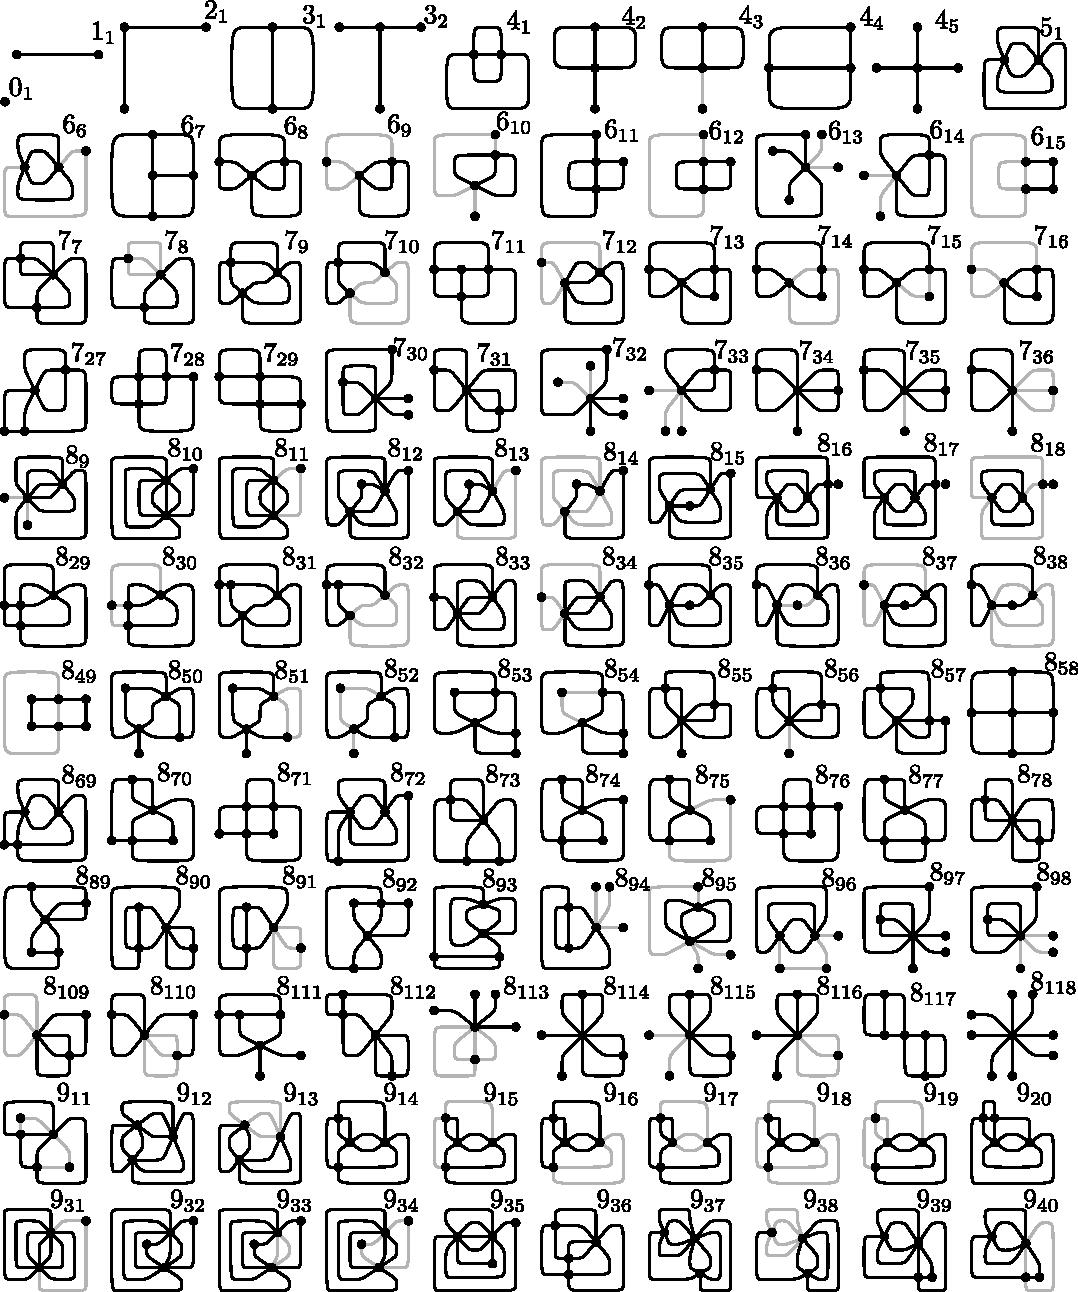
\includegraphics[width=16.5cm]{A.figs/primes489m11.pdf}} \eject \noindent
\subsection*{Part 1/4 in terms of blackboard framed links:}
\center{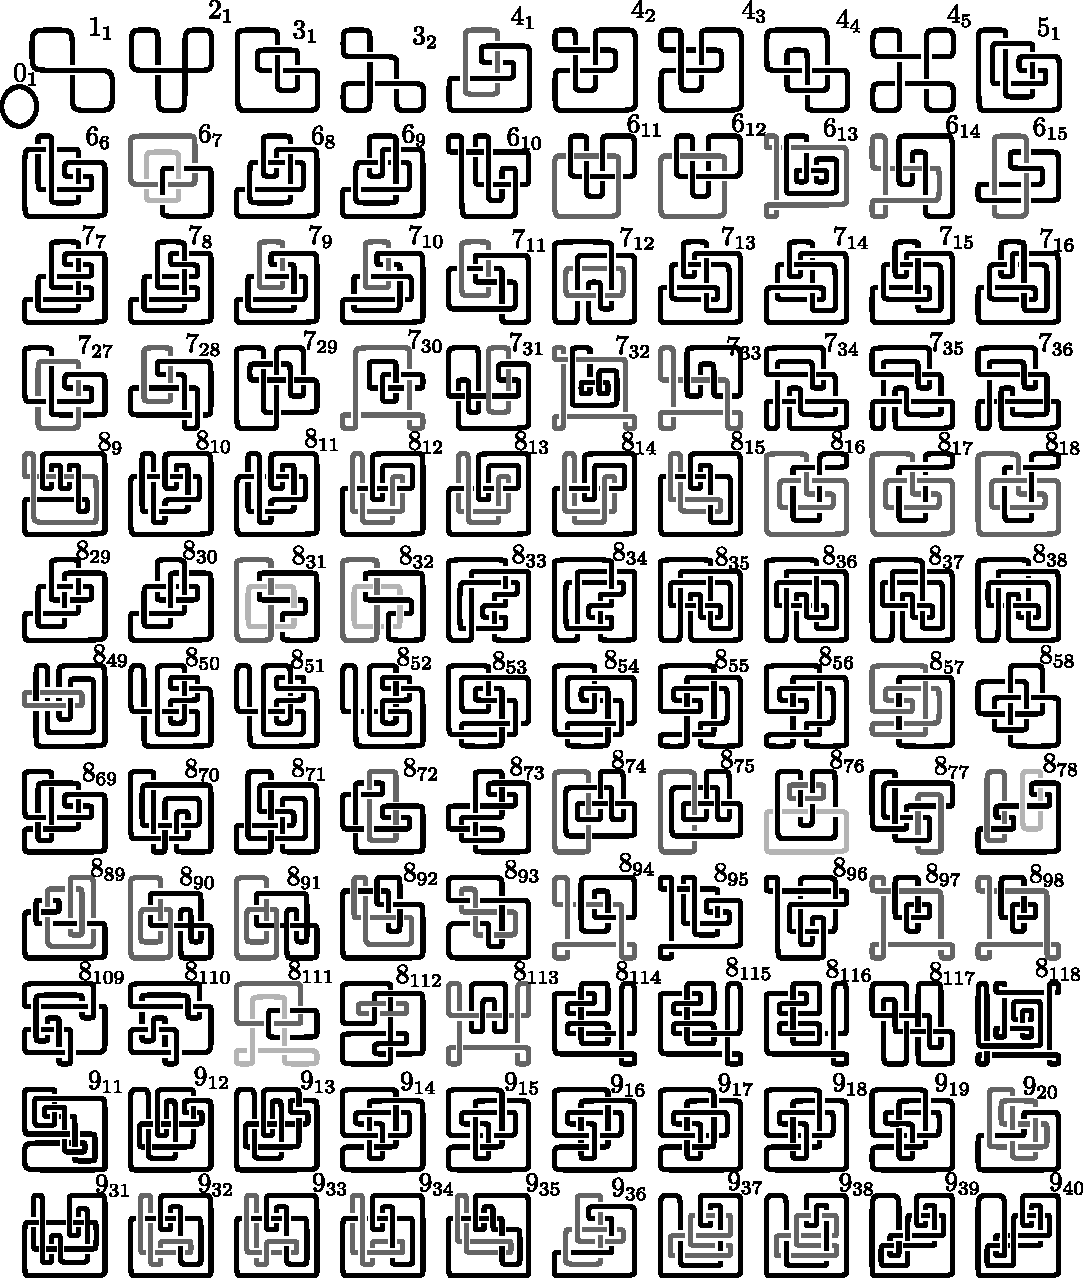
\includegraphics[width=16.5cm]{A.figs/primes489linksm11.pdf}} \eject
\subsection*{Part 2/4 in terms of blinks:}
\center{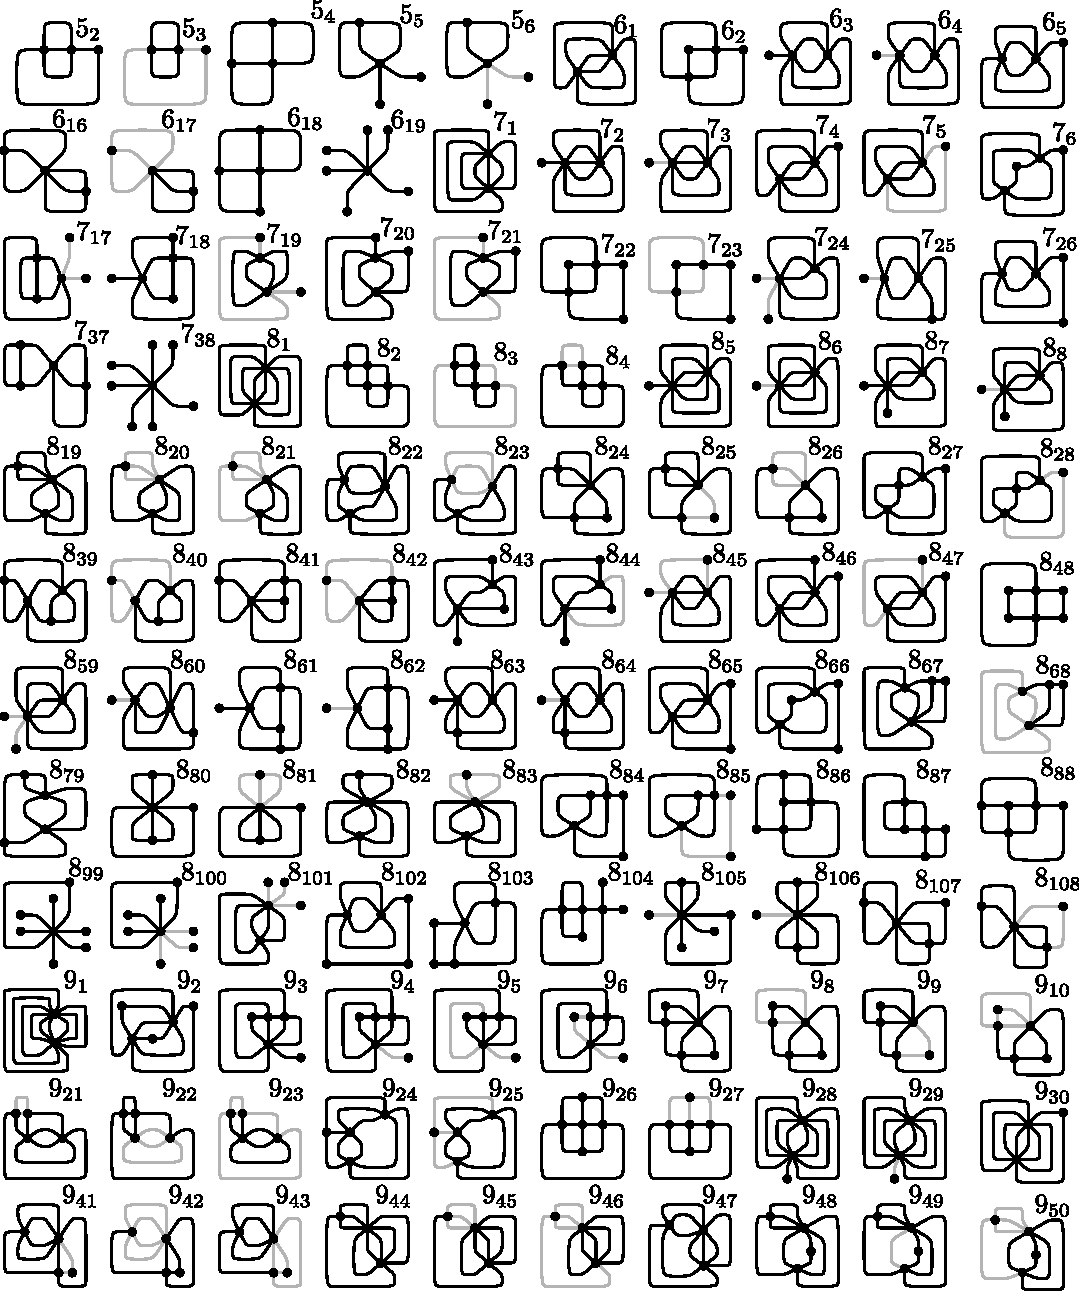
\includegraphics[width=16.5cm]{A.figs/primes489m12.pdf}} \eject
\subsection*{Part 2/4 in terms of blackboard framed links:}
\center{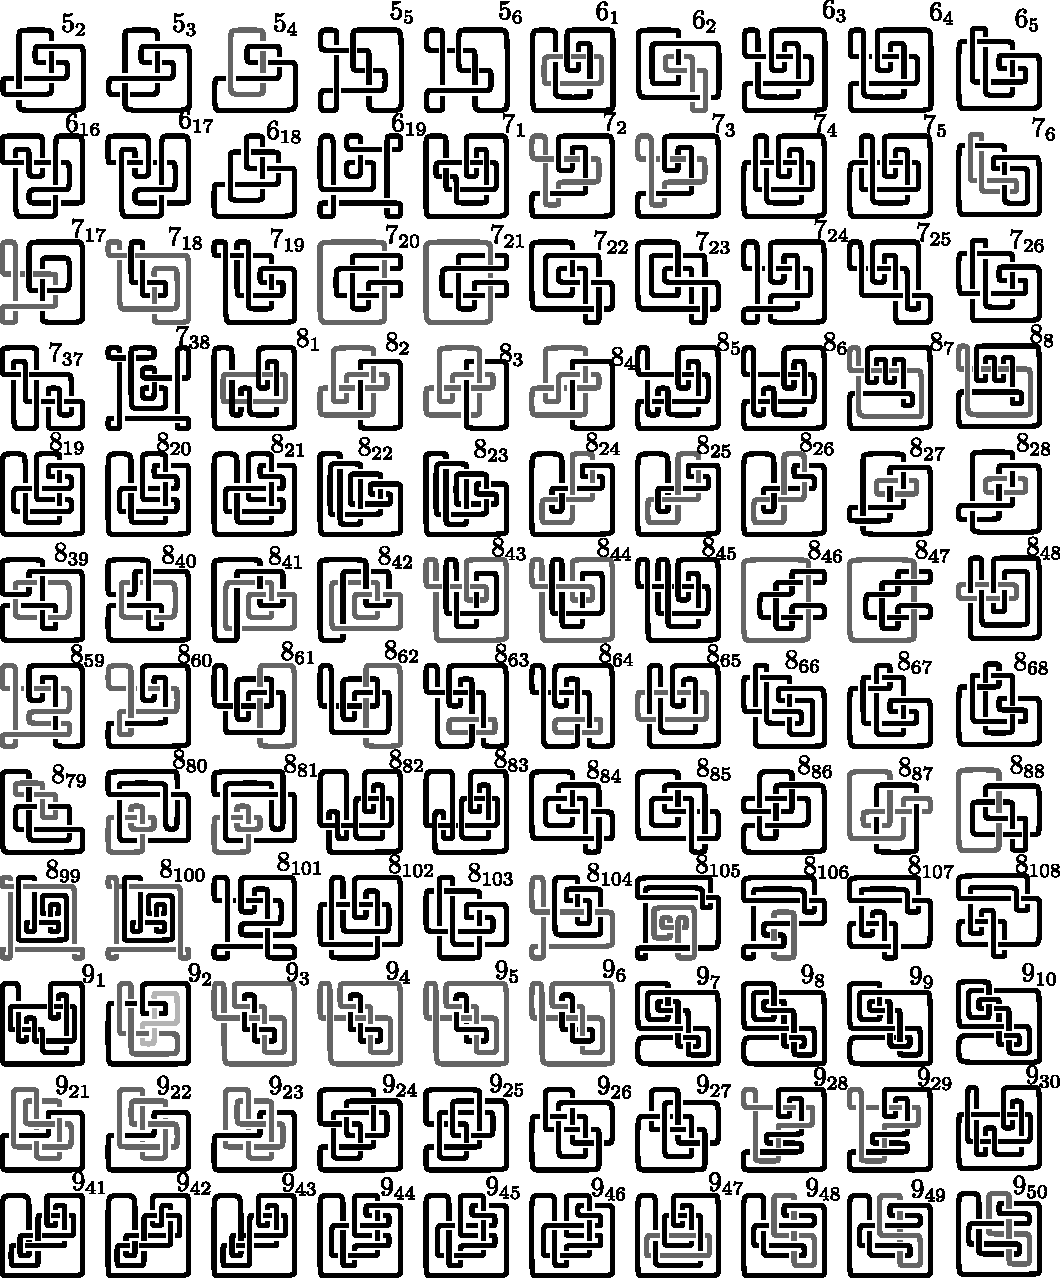
\includegraphics[width=16.5cm]{A.figs/primes489linksm12.pdf}} \eject
\subsection*{Part 3/4 in terms of blinks:}
\center{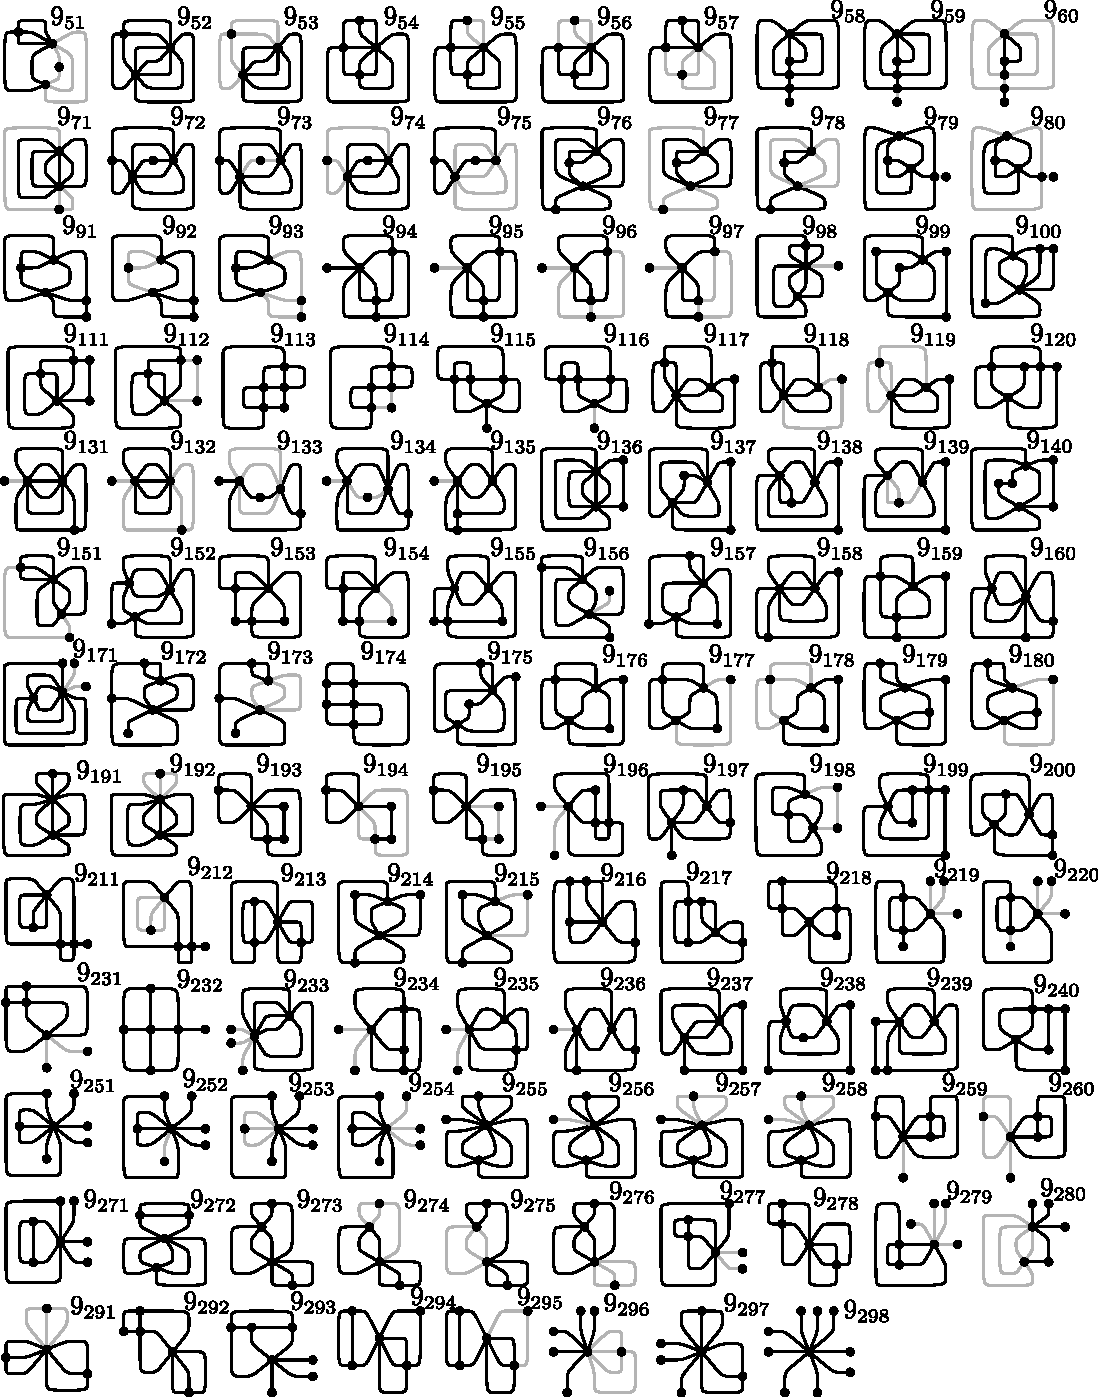
\includegraphics[width=16.5cm]{A.figs/primes489m21.pdf}} \eject
\subsection*{Part 3/4 in terms of blackboard framed links:}
\center{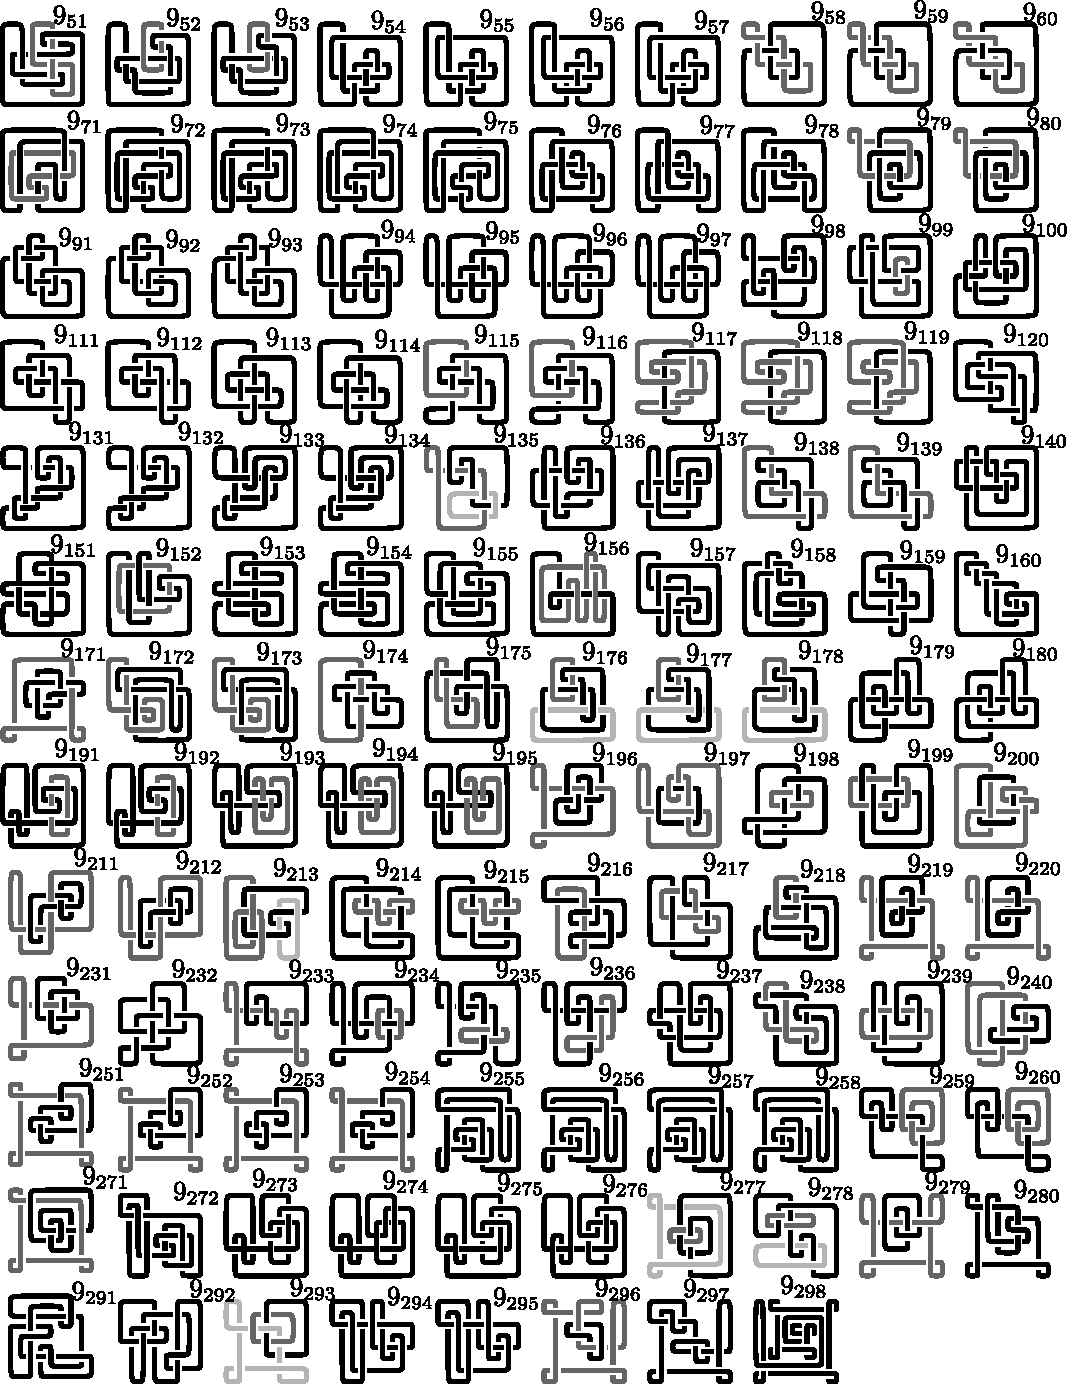
\includegraphics[width=16.5cm]{A.figs/primes489linksm21.pdf}} \eject
\subsection*{Part 4/4 in terms of blinks:}
\center{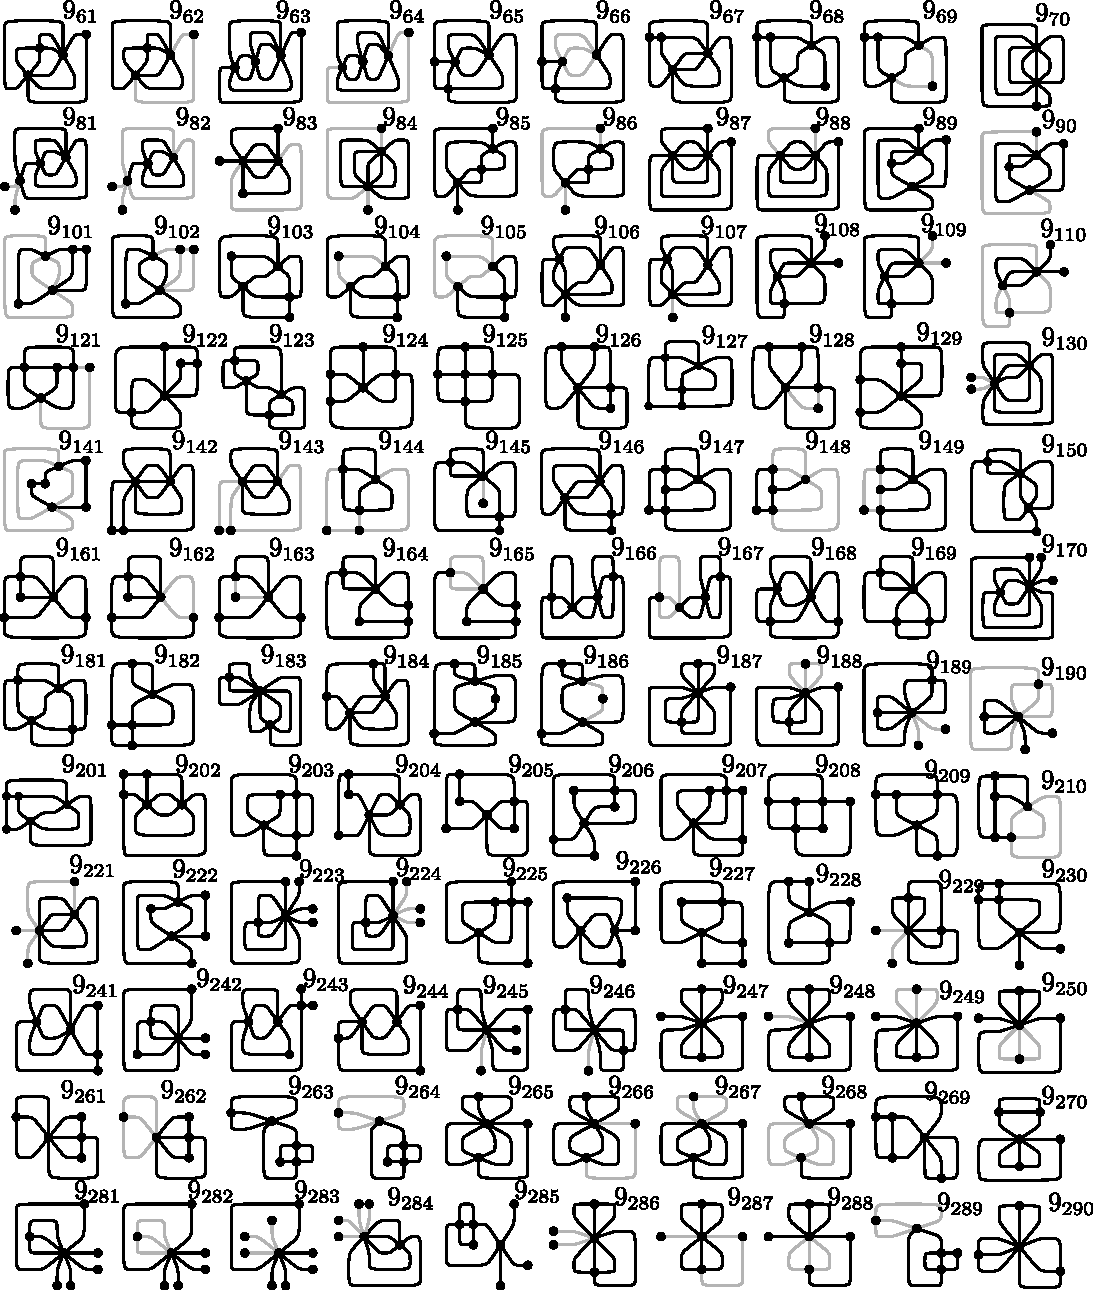
\includegraphics[width=16.5cm]{A.figs/primes489m22.pdf}} \eject
\subsection*{Part 4/4 in terms of blackboard framed links:}
\center{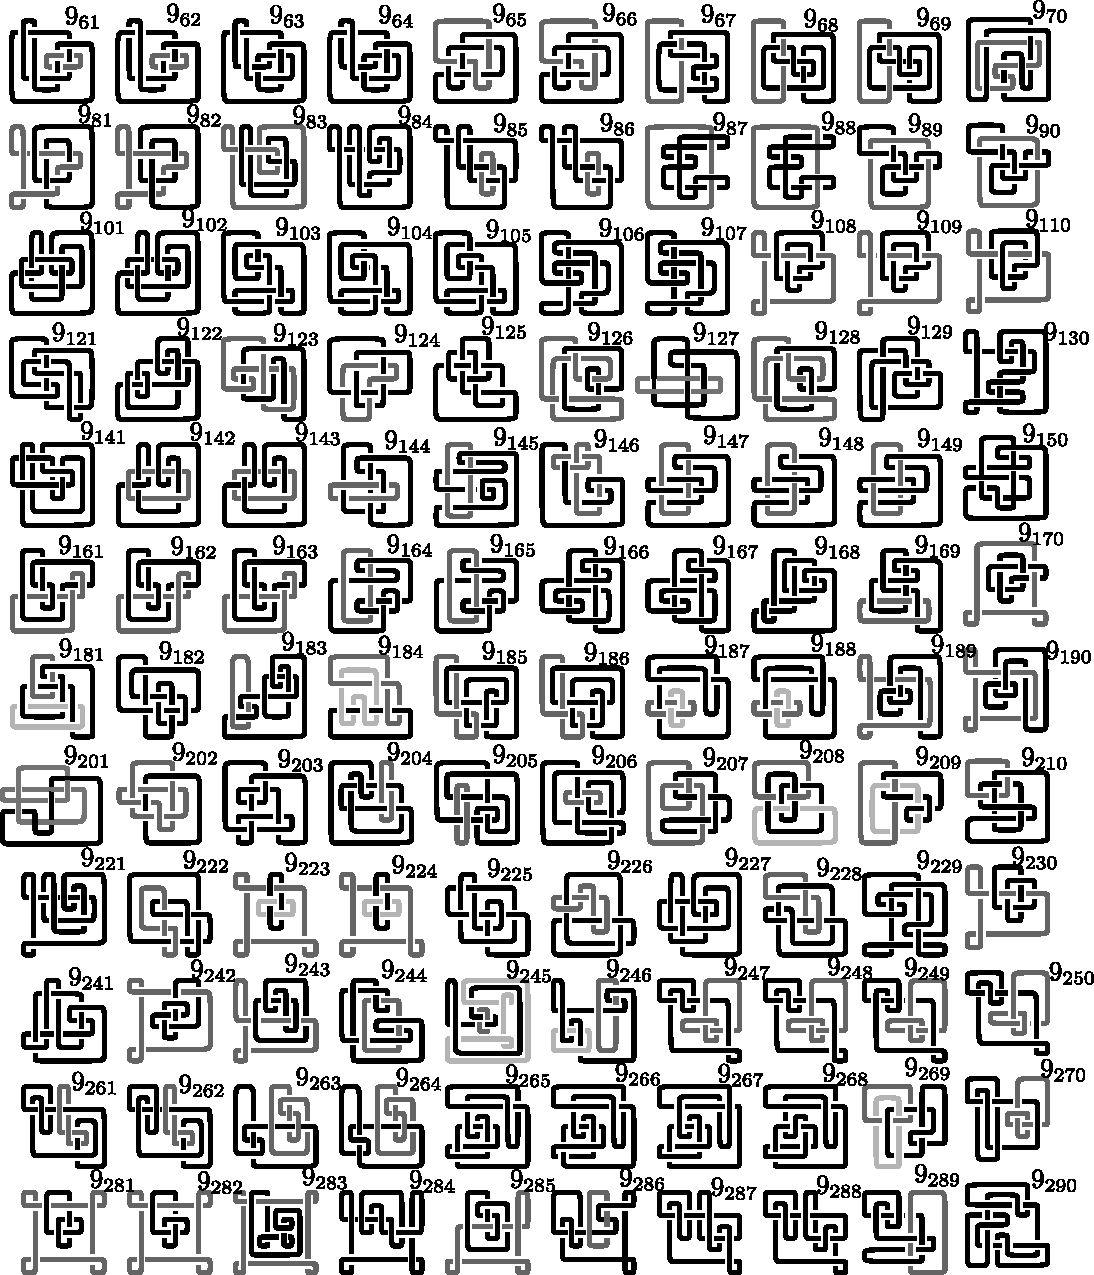
\includegraphics[width=16.5cm]{A.figs/primes489linksm22.pdf}}\eject


%-----------------------------------
\bibliographystyle{plain}
%\bibliographystyle{is-alpha}
%\addcontentsline{toc}{bibliografia}{\MakeTextUppercase{Refer�ncias Bibliogr�ficas}}
%\bibliography{d:/slsl\3.DadosSostenes.35.ArtigosLivros.bibtexGoogleScholar/bibtexIndex.bib} % bib file is slsl.bib
%\bibliography{~/home/ricardo/Dropbox/35.ArtigosLivros.bibtexGoogleScholar/bibtexIndex.bib}
\bibliography{bibtexIndex.bib}
%\bibliography{slsl}


\vspace{5mm}
\begin{center}
\hspace{7mm}
\begin{tabular}{l}
   S\'ostenes L. Lins\\
   Centro de Inform\'atica, UFPE \\
   Av. Jornalista Anibal Fernandes s/n\\
   Recife, PE 50740-560 \\
   Brazil\\
   sostenes@cin.ufpe.br
\end{tabular}
\hspace{20mm}
\hspace{7mm}
\begin{tabular}{l}
Lauro D. Lins\\
AT\&T Labs Research \\
180 Park Avenue \\
Florham Park, NJ 07932 \\
USA\\
llins@research.att.com
\end{tabular}
\hspace{20mm}

\end{center}


\end{document}

\begin{figure}[!htb]
\begin{center}
\includegraphics[scale=0.8]{A.figs/seconddoubt.pdf}
\caption{Are these 3-manifolds homeomorphic?}
\label{fig:seconddoubt}
\end{center}
\end{figure}

% \printindex
